\documentclass[letterpaper, 12pt]{article}
\usepackage{amsmath}
\usepackage[margin=1in]{geometry}
\usepackage{adjustbox}
\usepackage{graphicx}
\usepackage[final]{pdfpages}
\usepackage{bm}
\usepackage{sectsty}
\usepackage{titlesec}
\usepackage{lipsum}
\usepackage{subcaption}
\usepackage{listings}
\usepackage{pgffor}
\usepackage{rotating}
\usepackage{xcolor}  
\usepackage{amsthm}
\usepackage{csvsimple}
\usepackage{enumitem}
\usepackage{amssymb} 
\usepackage{amsfonts}
\usepackage{tikz}
\usepackage{tikz-3dplot}
% \setlength{\tabcolsep}{0.5cm} 
\newcommand{\thickhat}[1]{\mathbf{\hat{\text{$#1$}}}}
\renewcommand{\lstlistingname}{Program}

\newtheoremstyle{custom}
  {3pt}
  {3pt}
  {\itshape}
  {} 
  {\bfseries}
  {. }  
  { }   
  {\thmname{#1} \thmnumber{#2} \thmnote{ #3}}

\theoremstyle{custom}


\newtheorem{definition}{Definition}
% \newtheorem{theorem}{Theorem}
\newtheorem*{theorem}{Theorem}
\sectionfont{\fontsize{12}{15}\selectfont}
\titleformat{\section}
{\normalfont\normalsize\bfseries}
{(\thesection)}{1em}{}

\title{Laplace Transform of the Convolution Integral}
\date{}
\begin{document}
\maketitle
When we consider the Laplace transform, the convolution of two functions $f$ and $g$ is defined as

\begin{equation*}
  f*g = \int_{0}^{t} f(\tau) g(t - \tau) \, d\tau
\end{equation*}
Note that this definition differs from that used in the Fourier transform.

The Laplace transform of the convolution is given by
\begin{align*}
  \mathcal{L} \left[ f*g \right] 
  &= \int_{0}^{\infty} \int_{0}^{t} f(\tau) g(t-\tau) \, d\tau \, e^{-st} \, dt \\
  &= \int_{0}^{\infty} \int_{0}^{t} f(\tau) g(t-\tau) e^{-st} \, d\tau  \, dt
\end{align*}

We now perform the change of variables $\tau = u$, $t - \tau = v$,
which is equivalent to
\begin{align*}
  \tau &= u \\
  t &= u + v
\end{align*}

The integration region transforms as follows:
\begin{center}
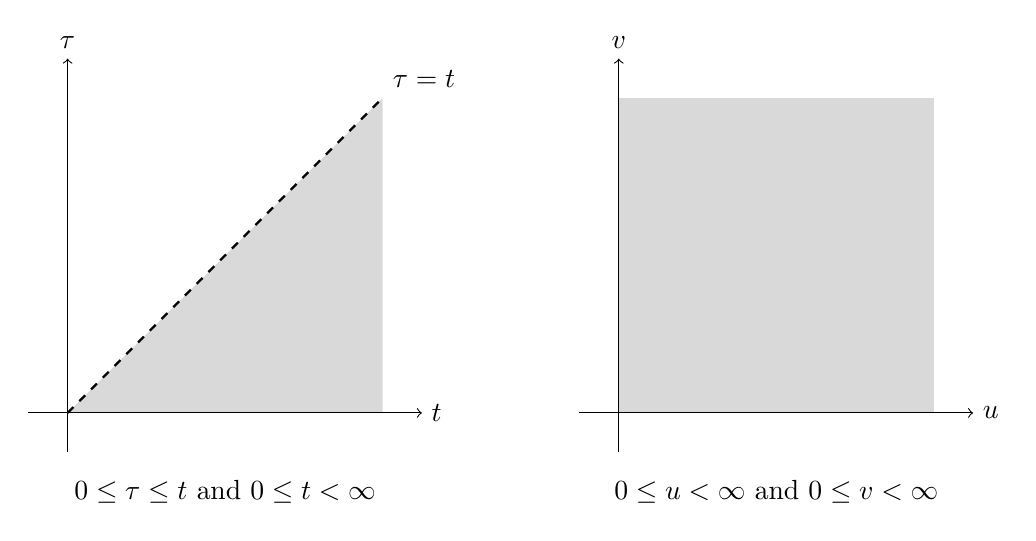
\begin{tikzpicture}

  \begin{scope}[shift={(0,0)}]
    \fill[gray!30] (0,0) -- (4,0) -- (4,4) -- cycle;
    \draw[->] (-0.5,0) -- (4.5,0) node[right] {$t$};
    \draw[->] (0,-0.5) -- (0,4.5) node[above] {$\tau$};
    \draw[thick, dashed] (0,0) -- (4,4) node[above right] {$\tau = t$};
    \node at (2,-1) {$0 \leq \tau \leq t$ and $0 \leq t < \infty$};
  \end{scope}
  
  \begin{scope}[shift={(7,0)}]
    \fill[gray!30] (0,0) -- (4,0) -- (4,4) -- (0,4) -- cycle;
    \draw[->] (-0.5,0) -- (4.5,0) node[right] {$u$};
    \draw[->] (0,-0.5) -- (0,4.5) node[above] {$v$};
    \node at (2,-1) {$0 \leq u < \infty$ and $0 \leq v < \infty$};
  \end{scope}
  
  \end{tikzpicture}
\end{center}

The determinant of the Jacobian matrix is 1.
Hence,
\begin{align*}
  \mathcal{L} \left[ f*g \right] 
  &= \int_{0}^{\infty} \int_{0}^{t} f(\tau) g(t-\tau) e^{-st} \, d\tau  \, dt \\
  &= \int_{0}^{\infty} \int_{0}^{\infty} f(u) g(v) e^{-s(u+v)} \, du  \, dv \\
  &= \int_{0}^{\infty} f(u) e^{-su} \, du \int_{0}^{\infty}  g(v) e^{-sv}  \, dv \\
  &= \mathcal{L} \left[ f \right] \mathcal{L} \left[ g \right] 
\end{align*}


\end{document}